\section{Introdução}\label{introduuxe7uxe3o}

Com a crescente adoção de equipamentos \iot (Internet of Things) para
monitoramento de sensores e acionamento de cargas, cresce também a
necessidade de ambientes de acompanhamentos de tais medições. Para isso
uma das melhores formas é usar a nuvem - recurso computacional sob
demanda através da internet \cite{ibm-cloud:2015} - para fazer o
armazenamento, já que uma das características dos equipamentos \iot é o
acesso à internet. Para atender essa necessidade surge a ideia de criar
um aplicativo web e livre que possa captar informações destes
dispositivos e que o acesso possa acontecer em qualquer lugar.

Equipamentos \iot são dispositivos com internet que podem se interligar
e se comunicar uns com os outros \cite{revell:2013}. Como exemplo temos
o Raspberry Pi que em quase 5 anos já vendeu 10 milhões de unidades pelo
mundo \cite{raspberry-pi-blog:2016}.

\section{Objetivos}\label{objetivos}

O objetivo principal do \wm é fornecer uma \emph{API} (\emph{Application
Program Interface}) leve, simples e segura, visto que equipamentos
\iot são limitados, para enviar e receber informações da nuvem.

Para que haja melhor intercâmbio das informações tanto partindo do
equipamento \iot quanto chegando, o protocolo de comunicação escolhido
foi o JSON (\emph{JavaScript Object Notation}), que segundo Douglas
Crockford é um formato leve e de linguagem independente para troca de
informações \cite{crockford:2015}.

\section{Justificativa}\label{justificativa}

Sendo um aplicativo de código-fonte licenciado pela GPLv3 (GNU Public
License) poderá ser usado tanto para professores e alunos de cursos
superiores e técnicos para estudo de microcontroladores, sistemas
embarcados e afins, como para empresas ou pessoas que queiram interagir
com seus equipamentos pessoais.

A linguagem de programação escolhida foi o PHP, a qual é fácil de
aprender, normalmente lecionada em cursos superiores e técnicos e de
hospedagem barata.

Outra característica a ser levada em conta é a forma de autenticação.
Uma autenticação convencional envolve a troca de \emph{cookies} entre
servidor e cliente, além de espaço em disco para guardar tais
informações. Em sistemas \iot que se supoem que possam crescer de forma
rápida, ou seja, o número de equipamentos pode aumentar, é necessário um
sistema de autenticação capaz de ser escalável mesmo em condições
limitadas. Para isso foi utilizado o padrão JWT (ou \emph{JSON Web
Tokens}), que é um padrão aberto (RFC 7519 \cite{rfc7519-2015}) que
define uma maneira compacta e auto-contida de transmitir de forma segura
informações entre pares através de um objeto JSON \cite{jwt-2016}. Esta
informação pode ser verificada e confirmada pois é assinada
digitalmente. Informações JWT podem ser assinadas usando um segredo (com
o algoritmo HMAC \cite{rfc2104-1997}) ou um par de chave pública e
privada usando RSA \cite{rfc3447-2003}.

\begin{figure}[h]
    \centering
    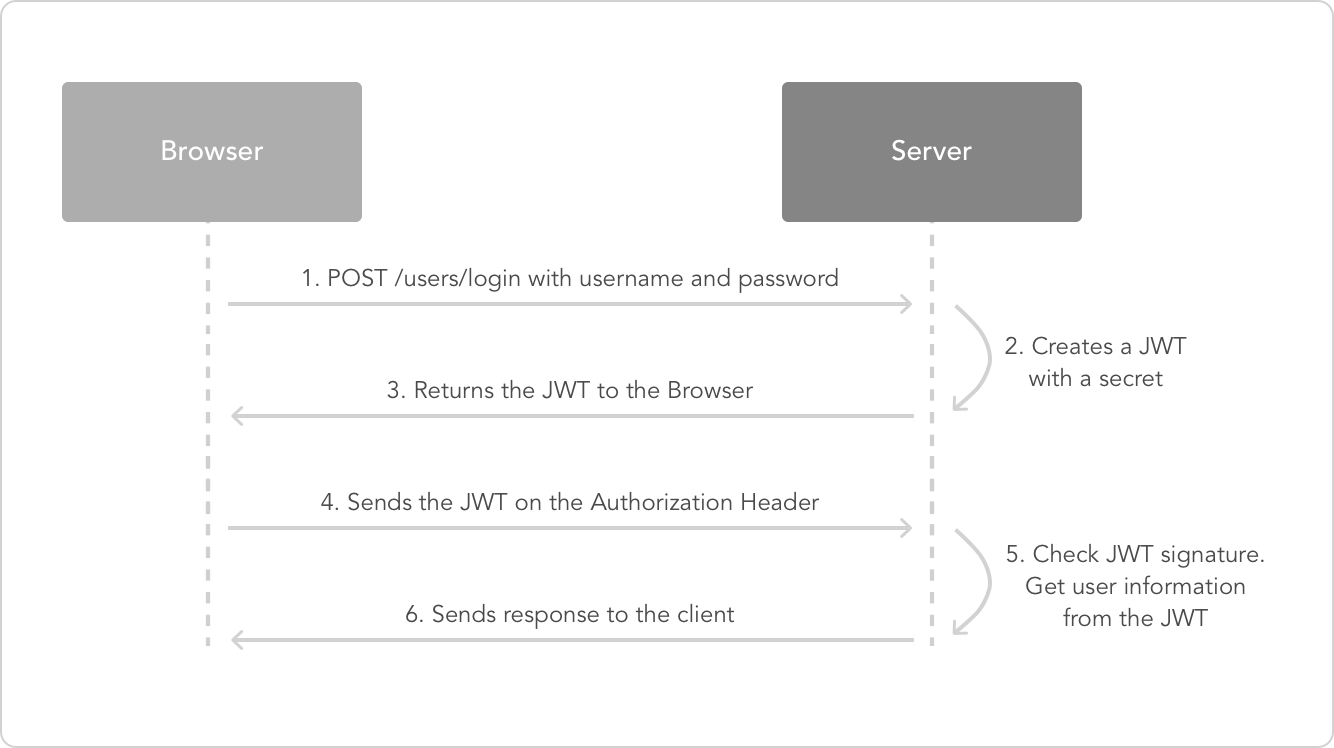
\includegraphics[scale=0.3]{img/jwt-diagram-grey.png}
    \caption{Diagrama do processo de autenticação - Fonte: https://cdn.auth0.com/content/jwt/jwt-diagram.png}
\end{figure}

\section{Revisão Teórica}\label{revisuxe3o-teuxf3rica}

Muitas são as soluções de monitoramento de equipamentos \iot. Podemos
citar as plataformas Oracle \iot, AWS \iot, Google Cloud \iot e
Microsoft Azure \iot Suite que são desenvolvidas por grandes empresas
como Oracle, Amazon, Google e Microsoft, respectivamente; até soluções
livres como Kaa, ThingSpeak, macchina.io, SiteWhere
\cite{postscapes-iot-2016}.

O grande desafio é permitir a extensão da ferramenta para necessidades
específicas. Ferramentas como o Kaa permitem criar módulos próprios,
sistemas de análises e modelo de dados, fazendo com que a ferramenta se
adapte ao que você precisa \cite{kaa-2014}.

De forma semelhante outras ferramentas como macchina.io oferecem opções
de criar \emph{bundles} \cite{macchina.io-2016}, o ThingSpeak oferece
opção de criar \emph{apps}, que podem envolver visualização em gráficos
e tomada de decisões \cite{thingspeak-2016}.

Nesse sentido a ferramenta proposta possui um sistema de plugins, que
são desenvolvidos como \emph{Laravel Packages}
\cite{laravel-packages-2016}. Cada nova funcionalidade é criada através
da ferramenta \emph{Laravel} e pode ser desenvolvida e habilitada
localmente.

A proposta é ter uma tela de acompanhamento dos dados captados do
equipamento que possam ser vizualizados de forma específica. A
documentação em português do brasil para criar um novo plugin pode ser
encontrada em
\url{https://sanusb-grupo.github.io/wireless-monitor/pt-br/plugin-development.html}.

\subsection{Comparativo com outras ferramentas
livres}\label{comparativo-com-outras-ferramentas-livres}

\begin{longtable}[c]{@{}llll@{}}
\toprule\addlinespace
\begin{minipage}[b]{0.22\columnwidth}\raggedright
Aplicativo
\end{minipage} & \begin{minipage}[b]{0.28\columnwidth}\raggedright
Ambiente do Servidor
\end{minipage} & \begin{minipage}[b]{0.25\columnwidth}\raggedright
Suporte a plugins
\end{minipage} & \begin{minipage}[b]{0.12\columnwidth}\raggedright
SDK
\end{minipage}
\\\addlinespace
\midrule\endhead
\begin{minipage}[t]{0.22\columnwidth}\raggedright
Kaa
\end{minipage} & \begin{minipage}[t]{0.28\columnwidth}\raggedright
Java
\end{minipage} & \begin{minipage}[t]{0.25\columnwidth}\raggedright
Sim
\end{minipage} & \begin{minipage}[t]{0.12\columnwidth}\raggedright
Sim
\end{minipage}
\\\addlinespace
\begin{minipage}[t]{0.22\columnwidth}\raggedright
macchina.io
\end{minipage} & \begin{minipage}[t]{0.28\columnwidth}\raggedright
C++/NodeJS
\end{minipage} & \begin{minipage}[t]{0.25\columnwidth}\raggedright
Sim
\end{minipage} & \begin{minipage}[t]{0.12\columnwidth}\raggedright
Sim
\end{minipage}
\\\addlinespace
\begin{minipage}[t]{0.22\columnwidth}\raggedright
SiteWhere
\end{minipage} & \begin{minipage}[t]{0.28\columnwidth}\raggedright
Java
\end{minipage} & \begin{minipage}[t]{0.25\columnwidth}\raggedright
Sim
\end{minipage} & \begin{minipage}[t]{0.12\columnwidth}\raggedright
Sim
\end{minipage}
\\\addlinespace
\begin{minipage}[t]{0.22\columnwidth}\raggedright
ThingSpeak
\end{minipage} & \begin{minipage}[t]{0.28\columnwidth}\raggedright
Ruby
\end{minipage} & \begin{minipage}[t]{0.25\columnwidth}\raggedright
Sim
\end{minipage} & \begin{minipage}[t]{0.12\columnwidth}\raggedright
Sim
\end{minipage}
\\\addlinespace
\begin{minipage}[t]{0.22\columnwidth}\raggedright
\wm
\end{minipage} & \begin{minipage}[t]{0.28\columnwidth}\raggedright
PHP
\end{minipage} & \begin{minipage}[t]{0.25\columnwidth}\raggedright
Sim
\end{minipage} & \begin{minipage}[t]{0.12\columnwidth}\raggedright
Não
\end{minipage}
\\\addlinespace
\bottomrule
\addlinespace
\caption{Comparativo com outras ferramentas \label{tab:comparativo}}
\end{longtable}

Como pode ser visto na Tabela \ref{tab:comparativo}, aplicativos como
Kaa e SiteWhere rodam em ambiente Java, o que encarece a implantação
devido a hospedagem ser mais cara comparada a hospedagem de aplicativos
PHP, bem como o poder de processamento deve ser elevado visto que tal
ambiente exige um servidor mais robusto.

Mesmo não possuindo um SDK (\emph{Software Development Kit}), para
auxilizar os desenvolvedores a utilizar o \wm, mas por ter um número
baixo de \emph{endpoint}'s e uma linguagem base bastante difundida e
suportada por um grande número de linguagens como no caso do JSON, não é
tão difícil criar funções de acesso a API.

Os \emph{endpoint}'s e suas descrições estão documentadas em
\url{https://sanusb-grupo.github.io/wireless-monitor/pt-br/api-endpoints/index.html}.

\section{Arquitetura}\label{arquitetura}

É necessário um servidor web, um equipamento \iot seja ESP8266 ou
Raspberry Pi com Arduino e um navegador de internet no cliente.

A arquitetura segue o modelo da Figura \ref{fig:arquitetura}, onde temos
o equipamento \iot que se comunica com o servidor através da internet
enviando um \emph{payload} no formato JSON e o cliente que busca os
dados recolhidos do servidor e exibe no navegador, \emph{desktop} ou
\emph{mobile}.

\begin{figure}[h]
    \centering
    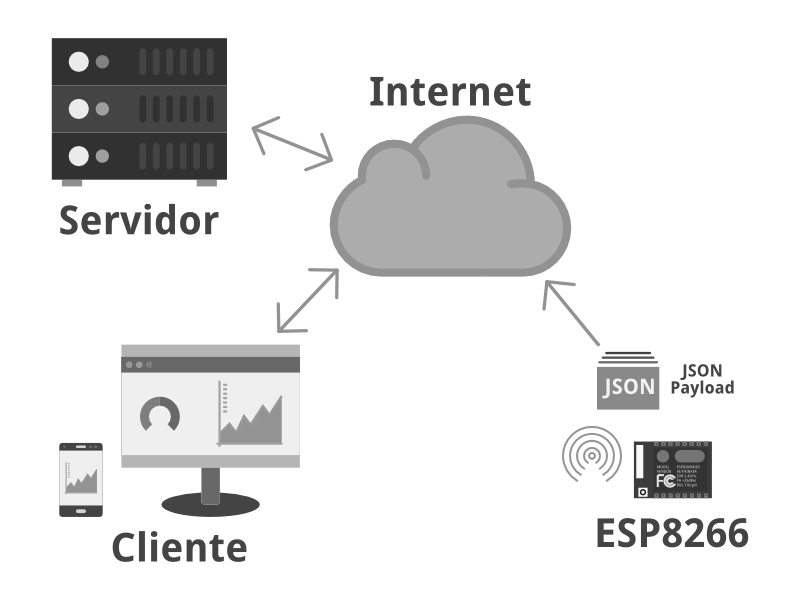
\includegraphics[scale=0.4]{img/arquitetura-grey.png}
    \caption{Arquitetura} \label{fig:arquitetura}
\end{figure}

\subsection{Servidor}\label{servidor}

No servidor deve existir uma instância do \wm, que trabalha em conjunto
com um banco de dados PostgreSQL, onde são armazenadas todas as
informações.

PostgreSQL é um ORDBMS (Object-relational database management system -
Sistema de Gerenciamento de Banco de Dados Objeto-relacional) baseado no
POSTGRES versão 4.2, desenvolvido na Universidade da Califórnia no
Departamento de Ciência da Computação de Berkley. POSTGRES foi pioneiro
em muitos conceitos que só se tornaram disponíveis em alguns sistemas de
bancos de dados comerciais muito tempo depois \cite{postgresql:2016}.

\section{Aplicação}\label{aplicauxe7uxe3o}

Nesta seção é mostrado um passo a passo de como o aplicativo funciona.

\subsection{Cadastro do desenvolvedor}\label{cadastro-do-desenvolvedor}

O desenvolvedor inicialmente deve fazer um cadastro simples no \wm
como pode ser visto na Figura \ref{fig:login-screen}. Esse cadastro irá
criar para ele uma \texttt{api\_key}, ou seja, uma chave única no
formato UUID 4 \cite{rfc4122:2005}.

\begin{figure}[h]
    \centering
    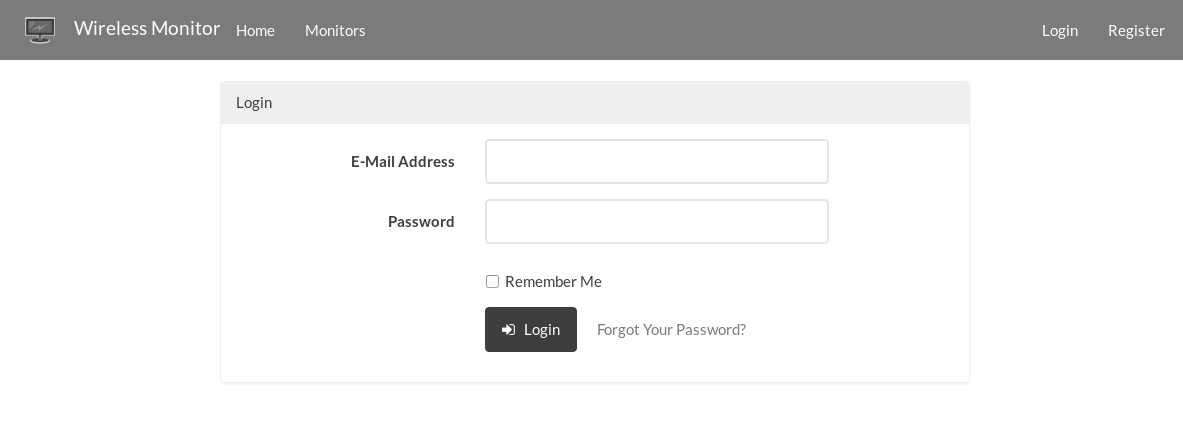
\includegraphics[scale=0.35]{img/login-screen-grey.png}
    \caption{Tela de Login} \label{fig:login-screen}
\end{figure}

\subsection{Criar um \emph{Monitor}}\label{criar-um-monitor}

Um \emph{Monitor} é um componente interno do sistema criado pelo
desenvolvedor de acordo com sua necessidade, é o instrumento que
caracteriza os dados coletados e os apresenta na interface web.

Imagine que o desenvolvedor queira medir a temperatura de um ambiente e
acompanhar suas variações. Para isso ele deve criar um \emph{Monitor} de
Temperatura, que apenas recebe um valor em intervalos de tempo. Dessa
forma o desenvolvedor pode acompanhar as variações ou ainda ver em forma
de gráfico um conjunto de variações de um período de tempo anterior.

De maneira análoga a criação de uma chave UUID para o desenvolvedor, uma
chave UUID é criada para o Monitor - \texttt{monitor\_key}.

As informações necessárias para criar um \emph{Monitor} de temperatura
podem ser visualizadas na Figura \ref{fig:new-temperature-monitor}.

\begin{figure}[h]
    \centering
    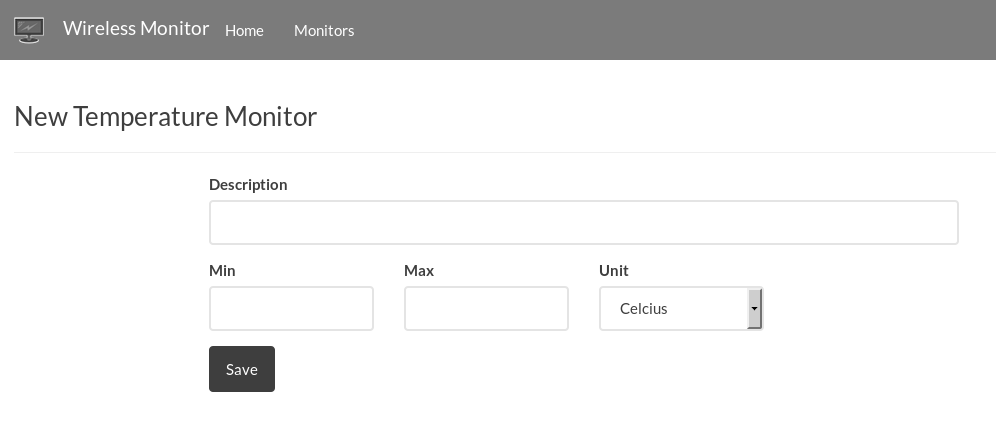
\includegraphics[scale=0.35]{img/new-temperature-monitor-grey.png}
    \caption{Novo Monitor de Temperatura} \label{fig:new-temperature-monitor}
\end{figure}

\subsection{Autenticação do
equipamento}\label{autenticauxe7uxe3o-do-equipamento}

Para autenticar e identificar o desenvolvedor e seu \emph{monitor} é
preciso enviar a \texttt{api\_key} e a \texttt{monitor\_key} via método
\emph{POST} para o \emph{endpoint} \texttt{/api/authenticate}. Em caso
positivo o sistema irá retornar um \emph{token}. Esse \emph{token}
servirá para qualquer troca de informações futuras entre o equipamento
\iot e o \wm.

Após ter o \emph{token} o desenvolvedor deve passá-lo através da
\emph{Header HTTP} denominada \emph{Authorization} usando \emph{schema
Bearer}. Algo do tipo:

\begin{verbatim}
Authorization: Bearer <token>
\end{verbatim}

Um \emph{token} é formado pelas seguintes informações:

\begin{itemize}
\itemsep1pt\parskip0pt\parsep0pt
\item
  \emph{Header}
\item
  \emph{Payload}
\item
  \emph{Signature}
\end{itemize}

Essa é uma forma segura e com pouco custo de memória. Além de ser uma
forma de autenticação \emph{stateless}, em que não são usadas sessões e
nem mesmo \emph{cookies}.

Para testar a autenticação fora do equipamento \iot é possível
utilizando a ferramenta \texttt{cURL}, que é uma ferramenta de linha de
comando e biblioteca para transferência de dados com sintaxe URL
\cite{curl:1996}.

\begin{verbatim}
curl -i -X POST \
    -F 'api_key=fa3076b3-ddb3-421f-a0ed-303a8dd04fb8' \
    -F 'monitor_key=e98fb37c-e79c-4a80-ac7f-b8fbdb82d48b' \
    http://localhost:8000/api/authenticate
\end{verbatim}

O servidor então responde informando o \emph{token}:

\begin{verbatim}
HTTP/1.1 200 OK
Date: Tue, 01 Oct 2016 23:34:29 GMT
Server: Apache
Cache-Control: no-cache
X-RateLimit-Limit: 60
X-RateLimit-Remaining: 59
Connection: close
Transfer-Encoding: chunked
Content-Type: application/json

{"token":"eyJ0eXAiOiJKV1QiLCJhbGciOiJIUzI1NiJ9.
eyJtb25pdG9yX2tleSI6ImU5OGZiMzdjLWU3OWMtNGE4MC1
hYzdmLWI4ZmJkYjgyZDQ4YiIsInN1YiI6MSwiaXNzIjoiaH
R0cDpcL1wvd2lyZWxlc3MtbW9uaXRvci5wcm92aXNvcmlvL
ndzXC9hcGlcL2F1dGhlbnRpY2F0ZSIsImlhdCI6MTQ3NjIy
ODg2OSwiZXhwIjoxNDc2MjMyNDY5LCJuYmYiOjE0NzYyMjg
4NjksImp0aSI6IjhhN2IwM2UxNGMzOThlYmEwZTJjZDU0ND
cwOTI5NDE2In0.hxuEY_F9lEg1UL0JA1FIIh0L1qw29WoMFLXAVLfeVo4"}
\end{verbatim}

\subsection{Envio dos dados}\label{envio-dos-dados}

Além do cabeçalho contendo o \emph{token} o usuário deve passar os
valores coletados pelo equipamento e enviar para o sistema. Para isso
ele deve enviar uma requisição \emph{POST} para o \emph{endpoint}
\texttt{/api/send}, com o atributo \texttt{data} contendo um JSON com os
dados.

No exemplo do \emph{Monitor} de temperatura é necessário enviar apenas o
valor, algo do tipo:

\begin{verbatim}
{
    "value": 23.89
}
\end{verbatim}

Usando o \texttt{cURL} a linha de comando deve ser algo como:

\begin{verbatim}
curl -i -X POST -H 'Content-Type: application/json' \
    -H 'Authorization: Bearer <TOKEN>' \
    -d '{"data":{"value":23.89}}' \
    http://localhost:8000/api/send
\end{verbatim}

Onde \texttt{\textless{}TOKEN\textgreater{}} deve ser substituído pelo
\emph{token} recebido da autenticação.

\subsection{Descrição dos
componentes}\label{descriuxe7uxe3o-dos-componentes}

Neste tópico são descritos os componentes e as ferramentas utilizadas
para o desenvolvimento e uso do plugin de Temperatura.

\subsubsection{Sistema embarcado linux}\label{sistema-embarcado-linux}

Foi utilizado a plataforma Raspberry Pi como sistema embarcado, que irá
servir para comunicação com o \wm e a plataforma Arduino. É um
equipamento \iot
capaz de interagir com outros dispositivos e com acesso à internet.

\subsubsection{Microcontrolador}\label{microcontrolador}

A plataforma Arduino foi escolhida para servir de ponte entre o
componente de medição de temperatura e o sistema embarcado.

Arduino é uma plataforma livre de eletrônica baseado em \emph{hardware}
e \emph{software} fáceis de usar. Placas Arduino são capazes de ler
entradas - luz em um sensor, controle usando botões, etc. - e converter
em uma saída - acionamento de um motor, acionamento de um LED,
publicação de dados online \cite{arduino:2016}.

\subsubsection{Sensor de temperatura}\label{sensor-de-temperatura}

Como sensor de temperatura foi usado o LM35 da Texas Instruments. A
série LM35 é composta de dispositivos de circuito integrado para medição
de temperatura com a tensão de saída linearmente proporcional a
temperatura em graus celsius. O sensor LM35 tem a vantagem sobre
sensores de temperatura linear calibrados em Kelvin, devido a não ser
necessário subtrair uma alta tensão constante da saída para obter uma
escala conveniente \cite{lm35:2016}.

\subsection{Ambiente de execução}\label{ambiente-de-execuuxe7uxe3o}

Para esse exemplo o ambiente de execução escolhido foi o NodeJS, que é
um envólucro (\emph{wrapper}) do ambiente de execução JavaScript de alta
performance chamado V8 usado no navegador Google Chrome. O NodeJS
permite que o V8 funcione em contextos diferentes do browser,
principalmente fornecendo APIs adicionais que são otimizadas para casos
específicos \cite{hughes-croucher:2012}. Por exemplo no caso de
equipamentos \iot é perfeito, pois se trata de um dispositivo orientado
a eventos, assim como o NodeJS.

Para auxiliar na conversação entre o NodeJS e o Arduino foi usado a
ferramenta Johnny-Five, uma plataforma livre Javascript para Robôs e
\iot \cite{johnny-five:2012}.

\subsection{Princípios de
execução}\label{princuxedpios-de-execuuxe7uxe3o}

O NodeJS deve ser instalado no Raspberry Pi já que possui suporte a
arquitetura ARM. Um projeto NodeJS deve ser criado tendo como
dependências o Johnny-Five e uma biblioteca de resquisições HTTP, como
por exemplo \texttt{request} \cite{request:2016}. Dessa forma o
Johnny-Five se encarregará de se comunicar com o Arduino requisitando a
temperatura do componente LM35. Com a resposta em mãos o NodeJS irá
enviar as medições ao Servidor através da biblioteca \texttt{request}.

O código fonte deste exemplo pode ser encontrado num repositório do
GitHub \cite{alves:2016} e a montagem do projeto pode ser vista na
Figura \ref{fig:montagem}, onde temos o Raspberry PI (1), o Arduino (2)
e o sensor de temperatura LM35 (3).

\begin{figure}[h]
    \centering
    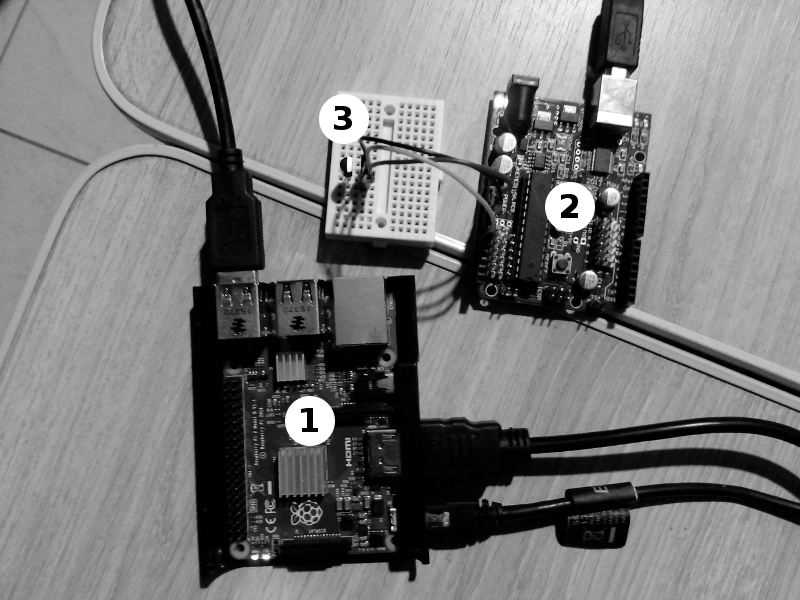
\includegraphics[scale=0.3]{img/montagem-grey.jpg}
    \caption{Montagem do projeto} \label{fig:montagem}
\end{figure}

\subsection{Visualização dos dados}\label{visualizauxe7uxe3o-dos-dados}

Após captar e enviar dados do \iot para a nuvem é possível acompanhar os
resultados pelo sistema. A forma de visualização será como mostra a
Figura \ref{fig:view-monitor}.

\begin{figure}[h]
    \centering
    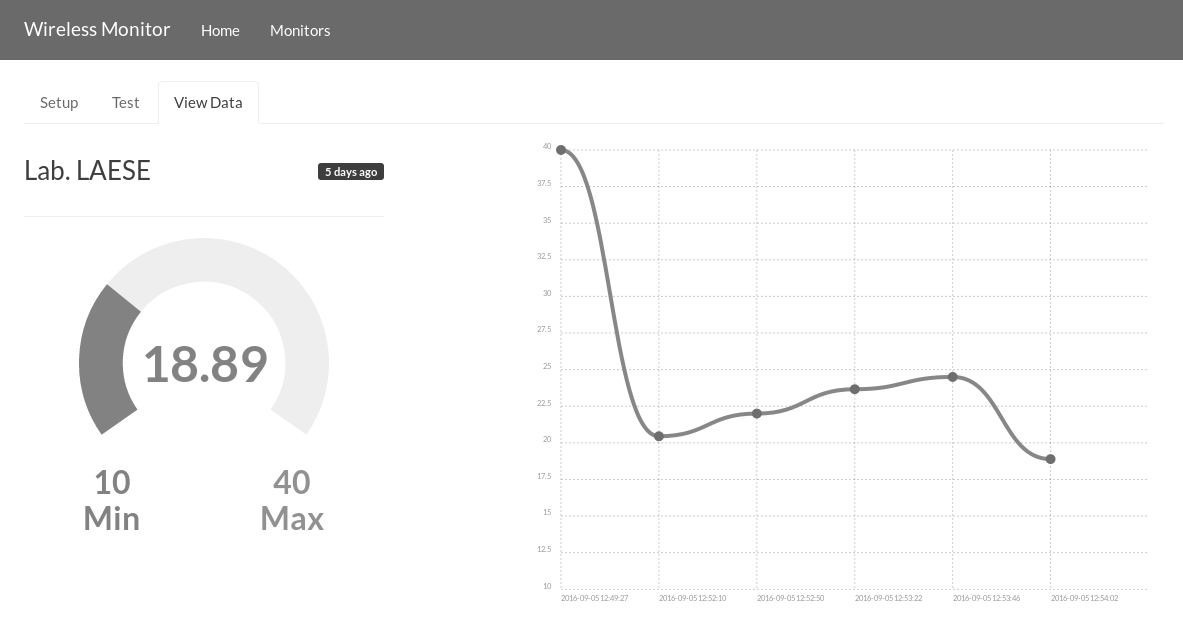
\includegraphics[scale=0.3]{img/temperature-show-grey.png}
    \caption{Visualização dos dados na web} \label{fig:view-monitor}
\end{figure}

\section{Conclusão}\label{conclusuxe3o}

A partir de ferramentas livres é possível criar ambientes de alta
qualidade para monitoramento de dispositivos \iot. Tanto porque grande
parte das ferramentas livres são estáveis e bem testadas, quanto pela
liberdade de poder customizar para que a ferramenta atenda as
necessidades dos envolvidos, diferentemente de ferramentas
proprietárias.

Um passo importante e que intimida um pouco é a forma de autenticação.
JWT é uma tecnologia muito recente e utiliza técnicas pouco
convencionais para o público iniciante, mas temos que levar em conta que
junto com o aumento do uso de equipamentos ligados à internet vem a
necessidade de segurança na comunicação. Uma falha de segurança que se
tornou comum nessas situações é chamada de \emph{man-in-the-middle}, que
pode ser definida como ``Uma falha de segurança em um computador em que
um usuário malicioso intercepta - e possivelmente altera - dados
trafegando em uma rede'' \cite{wordspy:2002}. Esse erro pode ocorrer
simplesmente porque os vínculos entre aparelhos e criptografias de
proteção cedidas por um padrão normalmente não foram implementadas
corretamente, como por exemplo em travas eletrônicas que usam Bluetooth
Low Energy (BLE) \cite{spring:2016}.

Uma prática comum para autenticação de \iot's é a criação de tokens
randômicos para identificar o usuário e o dispositivo, entretanto essa
técnica facilita o ataque \emph{man-in-the-middle}. Nessa linha o uso do
JWT possui vantagens quando comparado com um token randômico:

\begin{itemize}
\itemsep1pt\parskip0pt\parsep0pt
\item
  Chaves API randômicas não dizem nada a respeito do usuário, enquanto
  JWTs contém informações e metadados que descrevem a identidade do
  usuário; contém também uma validade por um período de tempo ou
  domínio.
\item
  JWT não obriga a necessidade um emissor de token centralizado ou
  autoridade de revogação de token.
\item
  É compatível com Oauth2 \cite{oauth2:2012}.
\item
  Dados do JWT podem ser inspecionados.
\item
  JWTs possuem controles de expiração \cite{romero:2015}.
\end{itemize}

Por fim o passo seguinte seria permitir o envio de comandos do navegador
para o dispositivo, podendo assim controlar algumas funcionalidades
remotamente como o acionamento de cargas, disparo de relés, entre outras
funções.
